% make title bold


\title{\textbf{A paper on Emin Alper's "Tepenin Ardı"}}
\author{
        RCTV Film Culture Final Exam\\
        Mustafa Cig Gokpinar - 19070001001\\
}
\date{\today}

\documentclass[12pt]{article}
\linespread{1.5}

\usepackage{graphicx}
\usepackage{url}
\usepackage{placeins}
\usepackage[margin=1in]{geometry}
\graphicspath{ {./images} }

\begin{document}
\maketitle

\section{Introduction}

\par
Emin Alper is Turkish filmmaker and screenwriter known for his thought-provoking films that explore social and political issues.
His 2012 film, "Tepenin Ardı" is a strong exploration of the impact on traditional ways of turkish life, the struggle between the individual and outer forces.
By drawing a portrait of a town in the midst of a conflict between the government and the local community over the construction of a hydroelectric dam, the film takes a look at the "enemy" figure.
In this paper, we will examine the biography and filmography of Emin Alper, the common themes and characters present in his work, and the cinematography techniques he employs.
We will also dive into the story and themes of "Tepenin Ardı" as well as analyzing the characters and their motivations.
\\

\section{About the Director}
\par
Emin Alper is born in Karaman in 1974. He enrolled into the Civil Engineering Department of Bogazici University, but he switched his major to pursue a career in economics and history. He now holds a Phd in Modern Turkish History from the Bogazici University.
\\
Since his adolescence years, Emin Alper was interested in movies. He had been jotting movie scripts and he was also a member of his university's cinema club. He spent most of his time in that club as an active member writing critiques and reviews. Invited famous turkish directors and actors to give speeches and workshops.
\\
His movie career officially started when he shot the first short film, "Mektup (2005)". Then, his first long feature film "Tepenin Ardı (20012)" was released. With the help of these successes he was now, known by the masses.
\\
To talk about his vision, one common theme in Emin Alper's films is the exploration of social and political issues. In "Tepenin Ardı" for example, the film examines the consequences of the Turkish government's construction and its impact on the local community. Another theme that can be seen is the human resilience of individuals in the face of threat.
\\
In terms of character development, Emin Alper often focuses on the portrayal of ordinary people and their struggles against the "enemy". Emin Alper generally plays on the "trust no one" theme, and his films often explore the complexities and flaws of his characters, as they struggle with their own personal enemiswhile trying to maintain their relationships with those around them. In Turkish society, it is common to see the "enemy" figure. As an foreigner, as the government, as the capitalist system, as the western culture... In short, as the "other". Emin Alper in "Tepenin Ardı" dives deep into this theme.
\\
Turkish cinema had a long debate on the role of "the father" or "the men", some directors pictured men as a strong and proud figure, some directors opposed and painted a picture of weak and vulnerable male characters. Some mocked the masculinity, some praised it. Emin Alper is one of the directors who played on the "toxic masculinity" theme, especially in the movie "Tepenin Ardı".
\\
Finally, to talk about Emin Alper's cinematography, his films often utilize natural lighting and landscapes to create a sense of nostalgia and sympathy for the characters.
In "Tepenin Ardı" for example, the film uses sweeping shots of the natural surroundings to convey the beauty of the village before the construction of the dam. The film also uses close-ups to emphasize the emotions of the characters.
One of the key cinematographical approaches that Emin Alper used specifically in "Tepenin Ardı" was to make the movie look western. He used a lot of western music, western style long shots, and editing techniques. This was again to emphasize the "other" theme
and the alienation of the villagers from the rest of the world.
\\

\begin{figure}[h]
        \begin{center}
                \includegraphics[width=80mm,scale=0.5]{Tepenin_Ardı}
                \caption{Tepenin Ardı (Emin Alper, 2012)}
        \end{center}
\end{figure}

\FloatBarrier

\section{About the Film}
\par
"Tepenin Ardı", Emin Alper's first feature length film, is a 2012 Turkish drama film both directed and written by Emin Alper himself. The film was a critical and commercial success, winning numerous awards at national and international film festivals, including the Berlin Film Festival. It examines the social and political issues of contemporary Turkey in a realistic manner, and is an exciting first step in Emin Alpers's career. The film takes place in a small village in Karaman, and follows the story of Faik (played by Tamer Levent), an elderly man living on his inherited land, and Nusret (played by Reha Özcan), who brings his two sons to visit their grandfather. What begins as a seemingly ordinary family reunion turns into a tragedy as Faik's increasing hatred towards the Yörük people, whom he accuses of stealing his goats and ruining his crops, leads to a series of events that escalate into violence.
\\
One of the central themes of the film is the dangers of hatred and discrimination. Faik's initial feelings towards the Yörük people, grow into a societal paranoia as he becomes into thinking the Yörük people as the enemy. This theme is elaborated even more to portray Faik, a figure of authority within the family, using his hatred towards the Yörük people to manipulate and exploit other family members. This theme can also be read as an allegory to contemporary Turkey, our country that has been a home to diverse groups of minorities with different languages and religions. However, unfortunately, always struggled from armed conflicts towards or in-between the groups. Mainly, These conflicts generally has 2 sides that present themselves as one dominant group that tries to impose its own identity on the minority group, leading to a sense of fear and insecurity within the minority group. This is clearly seen in the film, as Faik's family is subjected to a broken identity imposed by the dominant group, and their actions are driven by fear and insecurity.
\\
There is also a side of the movie that can be is as an allegory to the political situations in Turkey. The film is about the construction of a hydroelectric dam, which as we know constructions are always a controversial issue in Turkey, it causes many conflicts between the government and the locals. The film tries to understand the power dynamics in-between. This idea is later supported by depicting the government officials corrupt and willing to do anything to get what they want, even if it means hurting the locals.
\\
As you can see, these themes are very closely related to each other and Emin Alper used many different view-points to portray one of the oldest problems of the humankind. The weak vs the strong, the minority vs the majority, us vs "the others". First, the Yörüks vs the villagers. Then, the men vs the women. Finally, the government vs the locals. All of these conflicts are just different versions of the same problem, the power dynamics. Emin Alper, played his hand on this problem and filmed the movie in a realistic and objective way.

\begin{figure}[h]
        \begin{center}
                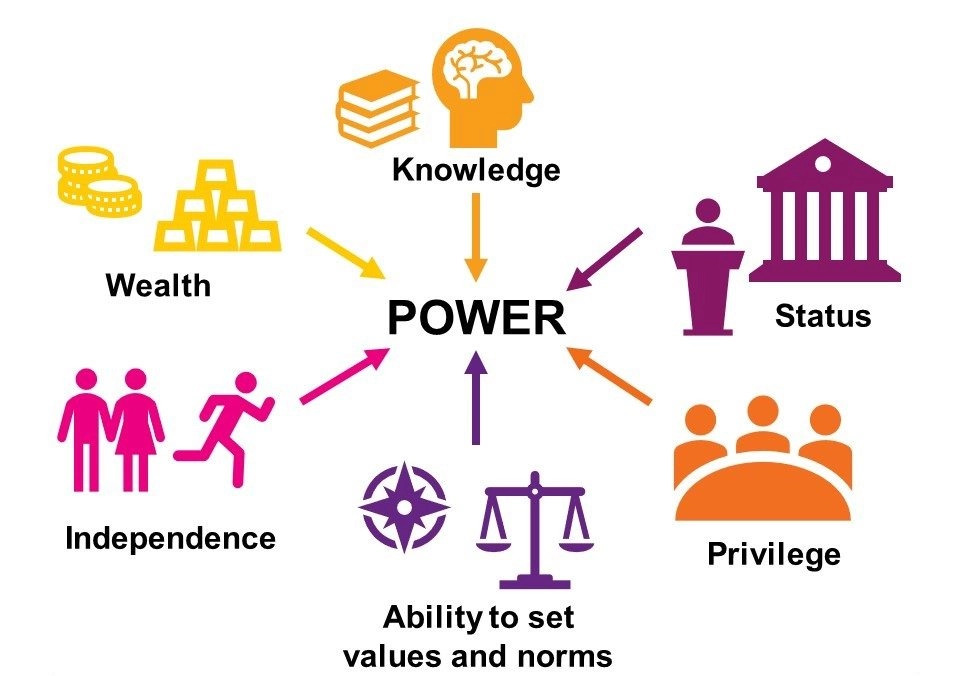
\includegraphics[width=120mm,scale=0.5]{power}
                \caption{The Power Dynamics (Power Dynamics in Writing Theory, 2019)}
        \end{center}
\end{figure}

\FloatBarrier

\par
Getting to the technical side, in terms of character development, the film focuses on the portrayal of Faik, Nusret, and the two sons. Faik is a masculine and conservative character, whose motives are driven by his feelings of hate towards the Yörük people and instincts to protect his land. Nusret, on the other hand, is a more understanding character, who tries to defuse the conflict between Faik and the Yörük people and maintain peace within the family. The two sons, play important roles in the film to make the plot go deeper and later unfold.
\\
\par
Overall, "Tepenin Ardı" is a film that explores themes of hatred, discrimination, and power dynamics through the portrayal of its characters. Through its allegories of Turkey, the film is a commentary on the social and political issues of our time. The film's naturalistic cinematography, which captures the beauty and tranquility of the village before the construction of the dam, serves a purpose tell get the viewers into the emotional impact of the story and immerse them. Also, the western look is used to emphasize the "other" theme and the alienation of the villagers from the rest of the world. The film is a great example of how a director can use the power of cinema to tell a story and make a statement on our society.

\section*{References}

% numbered list
\begin{enumerate}
        \item Tepenin Ardı. (n.d.). Beyazperde. \url{https://www.beyazperde.com/filmler/film-203102/}
        \item Wikipedia contributors. (2015, September 10). Emin Alper. Vikipedi. \url{https://tr.wikipedia.org/wiki/Emin_Alper}
        \item Wikipedia contributors. (2012, October 28). Tepenin Ardı. Vikipedi. \url{https://tr.wikipedia.org/wiki/Tepenin_Ard%C4%B1}
        \item Yoksu, E. K. (2021, January 24). Mükemmel sinematografiye sahip 15 yerli film. Independent Türkçe. \url{https://www.indyturk.com/node/304846/t%C3%BCrki%CC%87yeden-sesler/m%C3%BCkemmel-sinematografiye-sahip-15-yerli-film}
        \item Düşova, E. (2019, May 9). Bir Düşmanlık Alegorisi: Tepenin Ardı (2012). Fil’m Hafızası. \url{https://filmhafizasi.com/bir-dusmanlik-alegorisi-tepenin-ardi-2012/}
        \item Power Dynamics in Writing Theory. (2019, November 3). Peace and Quiet. \url{https://lindapham2019.wordpress.com/2019/11/03/power-dynamics-and-writing-theory/}
\end{enumerate}
\end{document}
